\RequirePackage{silence} % :-\
  \WarningFilter{scrreprt}{Usage of package `titlesec'}
  \WarningFilter{titlesec}{Non standard sectioning command}
\documentclass[11pt,
  footinclude,headinclude,
  abstract=on
]{scrreprt}
%paper=b5

%% %%%%%%%%%%%%%%%%%%%%%%%%%%%%%%%%%%%%%%%%%%%%%%%%%%%%%%%%%%%%%%%%%%%%%%
%% ************************************************************
%% ==================================================

%% General
%% %%%%%%%%%%%%%%%%%%%%%%%%%%%%%%%%%%%%%%%%%%%%%%%%%%%%%%%%%%%%%%%%%%%%%%

\usepackage[T1]{fontenc}
\usepackage[linedheaders=true]{classicthesis} % ,manychapters
%\usepackage[osf]{libertine}
\usepackage[english]{babel}

%% Bibliography
%% %%%%%%%%%%%%%%%%%%%%%%%%%%%%%%%%%%%%%%%%%%%%%%%%%%%%%%%%%%%%%%%%%%%%%%

\usepackage{natbib}
%% Settings copied from the ACM style
\bibliographystyle{ACM-Reference-Format}{}
\setcitestyle{%
    authoryear,%
    open={[},close={]},citesep={;},%
    aysep={},yysep={,},%
    notesep={, }}
\let\citeN\cite
\let\cite\citep

%% Style
%% %%%%%%%%%%%%%%%%%%%%%%%%%%%%%%%%%%%%%%%%%%%%%%%%%%%%%%%%%%%%%%%%%%%%%%

\usepackage{xspace}
\usepackage{xcolor}

%% Math
%% %%%%%%%%%%%%%%%%%%%%%%%%%%%%%%%%%%%%%%%%%%%%%%%%%%%%%%%%%%%%%%%%%%%%%%



\begin{document}

%% General
%% ======================================================================

\newcommand{\TODO}[1]{\textcolor{red}{\textbf{TODO:} #1}}

\newcommand{\figref}[1]{Fig.~\ref{#1}\xspace}
\newcommand{\lemref}[1]{Lem.~\ref{#1}\xspace}
\newcommand{\thmref}[1]{Thm.~\ref{#1}\xspace}
\newcommand{\ruleref}[1]{Rule~{\small #1}\xspace}
\newcommand{\defref}[1]{Def.~\ref{#1}\xspace}
\newcommand{\secref}[1]{Section~\ref{#1}\xspace}
\newcommand{\chapref}[1]{Chapter~\ref{#1}\xspace}
\newcommand{\appref}[1]{Appendix~\ref{#1}\xspace}

\newcommand{\tdef}[1]{\textbf{#1}}

\newcommand{\CSharp}{C\texttt{\small\#}\xspace}
\newcommand{\FSub}{$F^N_{\leq}$\xspace}

%% for wide figures:
%% http://16marzo.blogspot.com/2009/09/figure-e-margini-in-classicthesis.html
\newlength\largefigure
\setlength{\largefigure}{\columnwidth+\marginparsep+\marginparwidth}

\definecolor{light-gray}{gray}{0.85}

\newcommand{\cfbox}[2]{%
    \colorlet{currentcolor}{.}%
    {\color{#1}%
    \fbox{\color{currentcolor}#2}}%
}

%% Code
%% *********************************************************

\newcommand{\code}[1]{\texttt{\small#1}\xspace}
\newcommand{\cjl}[1]{\lstinline[language=Julia]!#1!\xspace}

\lstnewenvironment{julia}
    {\lstset{language=Julia,numbers=left,}}
    {}
\newenvironment{codeenvd}
    {
    \begin{center}
    \begin{minipage}{8cm}
    }
    {
    \end{minipage}
    \end{center}
    }

%% Math
%% *********************************************************

%% make sure we are in math mode
\newcommand{\EM}[1]{\ensuremath{#1}\xspace}

\newtheorem{theorem}{Theorem}
\newtheorem{lemma}{Lemma}

\newcommand{\interp}[1]{\EM{\llbracket #1 \rrbracket}}

%% Formalization
%% ======================================================================

%% Metavariables
%% *********************************************************

\newcommand{\ty}{\EM{\tau}}                 %% type annotation τ
\newcommand{\gty}{\EM{\sigma}}              %% type tag σ

\newcommand{\nsty}{\EM{\phi}}               %% normalized simple type φ
%% normalized existential type
\newcommand{\nety}{\EM{\xi}}
%\newcommand{\nety}{\EM{\prescript{\exists}{}{\phi}}}        %% ∃φ
%% normalized union-existential type
\newcommand{\nuty}{\EM{\omega}}
%\newcommand{\nuty}{\EM{\prescript{}{\cup\exists}{\phi}}}    %% ∪∃φ       


\newcommand{\cname}{\EM{\mathit{cname}}}
\newcommand{\aname}{\EM{\mathit{aname}}}
\newcommand{\iname}{\EM{\mathit{name}}}

\newcommand{\VEnv}{\EM{\mathrm{V}}}     %% simple variable environment V
\newcommand{\AEnv}{\EM{\Gamma}}         %% forall-variable environment Γ
\newcommand{\EEnv}{\EM{\mathbf\Delta}}         %% exist-variable environment Δ
                                        %% (unification variables)
\newcommand{\EmptyEnv}{\EM{\cdot}}

\newcommand{\CSet}{\EM{\mathcal{C}}}    %% set of subtype constraints
\newcommand{\EmptySet}{\EM{\varnothing}}    %% empty set of constraints

%% Style
%% *********************************************************

\newcommand{\tyname}[1]{\EM{\mathsf{#1}}}       %% type name (like Int)
\newcommand{\var}[1]{\EM{\mathrm{#1}}}          %% type variable
\newcommand{\unvar}[1]{\EM{\mathbf{#1}}}        %% unification variable

%% overline for list
\newcommand{\ol}[1]{\EM{\overline{#1}}}

%% set
\newcommand{\cset}[1]{\EM{\{#1\}}}

%% side condition
\newcommand{\sidecond}[1]{\EM{\scriptstyle #1}}

%% inference rule names
\newcommand{\SR}[1]{\textsc{S-#1}}
\newcommand{\ER}[1]{\textsc{E-#1}}

%% Symbols
%% *********************************************************

\newcommand{\Alt}{~\vert~}                      %% |

\newcommand{\symsub}{\EM{<:}}                   %% <:
\newcommand{\symeq}{\EM{\approx}}               %% ==
%\newcommand{\vdashfr}{\EM{\vdash\!\!{\circ}}}   %% |-o
\newcommand{\vdashfr}{\EM{\Vdash}}   %% ||-

%% Type Constructors
%% *********************************************************

\newcommand{\tyany}{\tyname{Any}}               %% Any
\newcommand{\tybot}{\tyname{Bot}}               %% Bot

\newcommand{\typair}[2]{\EM{#1 \times #2}}      %% t1 × t2
\newcommand{\tyunion}[2]{\EM{#1 \cup #2}}       %% t1 ∪ t2

\newcommand{\tyinv}[2]{\EM{#1\{#2\}}}           %% t1{...}

%\newcommand{\tybound}[3]{\EM{\tyvar{#1}\!\in\!({#2},{#3})}} %% X \in (tl,tu)
\newcommand{\varbound}[3]{\EM{#2\!\symsub\!#1\!\symsub\!#3}} %% tl<:X<:tu
\newcommand{\tybound}[3]{\varbound{\tyvar{#1}}{#2}{#3}} %% tl<:X<:tu
\newcommand{\tyboundu}[2]{\EM{\tyvar{#1}\!\symsub\!#2}}     %% X<:tu
\newcommand{\gtybound}[2]{\EM{\gtyvar{#1}\!\symsub\!#2}}    %% X<:tu
%\newcommand{\untybound}[3]{\EM{\tyvar{\unvar{#1}}\!\in\!({#2},{#3})}} %% Q \in
%(tl,tu)
\newcommand{\untybound}[3]{\EM{#2\!\symsub\!\tyvar{\unvar{#1}}\!\symsub\!#3}} %% tl<:Q<:tu
\newcommand{\ungtybound}[2]{\EM{\gtyvar{\unvar{#1}}\!\symsub\!#2}}    %% Q<:tu

%% regular existential type with all bounds ∃tX_lb^ub.t
\newcommand{\tyexist}[4]{\EM{\exists\tybound{#1}{#2}{#3}.#4}}
%% concrete existential type withh all bounds ∃gX^ub.t
\newcommand{\gtyexist}[3]{\EM{\exists\gtybound{#1}{#2}.#3}}
%% regular existential type with only upper bound ∃tX^ub.t
\newcommand{\tyexistu}[3]{\EM{\exists\tyboundu{#1}{#2}.#3}}
%% regular existential type with no bounds ∃tX.t
\newcommand{\tyexistnb}[2]{\EM{\exists\tyvar{#1}.#2}}
%% concrete existential type with no bounds ∃gX.t
\newcommand{\gtyexistnb}[2]{\EM{\exists\gtyvar{#1}.#2}}
%% simple existential type with no bounds ∃X.t (variable kind is not specified)
\newcommand{\styexist}[2]{\EM{\exists\var{#1}.#2}}

%% lists of types
\newcommand{\tys}{\EM{\ol{\ty}}}
\newcommand{\gtys}{\EM{\ol{\gty}}}
\newcommand{\nutys}{\EM{\ol{\nuty}}}

%% closed types
\newcommand{\closed}[1]{\EM{\dot{#1}}}
\newcommand{\cty}{\closed{\ty}}
\newcommand{\cgty}{\closed{\gty}}
\newcommand{\cnuty}{\closed{\nuty}}

\newcommand{\tyvar}[1]{\var{\prescript{\circ}{}{#1}}}     %% type variable
\newcommand{\gtyvar}[1]{\var{\prescript{\bullet}{}{#1}}}   %% concrete type variable
\newcommand{\avar}[1]{\var{\prescript{?}{}{#1}}}        %% any type variable

%% constraints
\newcommand{\subctr}[2]{\EM{#1 \leq #2}}
\newcommand{\eqctr}[2]{\EM{#1 = #2}}

%% %%%%%%%%%%%%%%%%%%%%%%%%%%%%%%%%%% Type Examples

\newcommand{\tyint}{\tyname{Int}}
\newcommand{\tyflt}{\tyname{Flt}}
\newcommand{\tystr}{\tyname{Str}}

\newcommand{\nref}{\tyname{Ref}}
\newcommand{\ninvpair}{\tyname{Pair}}

\newcommand{\vx}{\var{X}}
\newcommand{\vy}{\var{Y}}

\newcommand{\tvx}{\tyvar{X}}
\newcommand{\tvy}{\tyvar{Y}}

\newcommand{\gvx}{\gtyvar{X}}
\newcommand{\gvy}{\gtyvar{Y}}

\newcommand{\avx}{\avar{X}}
\newcommand{\avy}{\avar{Y}}

\newcommand{\uavq}{\avar{\unvar{Q}}}
\newcommand{\utvq}{\tyvar{\unvar{Q}}}
\newcommand{\ugvq}{\gtyvar{\unvar{Q}}}

%% Meta functions
%% *********************************************************

\DeclareMathOperator{\fvop}{\mathit{FV}}
\DeclareMathOperator{\domop}{\mathit{dom}}

\DeclareMathOperator{\ubop}{\mathit{ub}}    %% upper bound
\DeclareMathOperator{\lbop}{\mathit{lb}}    %% lower bound

\DeclareMathOperator{\normop}{\mathsf{Norm}}
\DeclareMathOperator{\solvecop}{\mathbf{Solve}}

\newcommand{\fv}[1]{\EM{\fvop(#1)}}
\newcommand{\dom}[1]{\EM{\domop(#1)}}

\newcommand{\ub}[2]{\EM{\ubop(#1, #2)}}
\newcommand{\ubd}[1]{\ub{\AEnv}{#1}}
\newcommand{\lb}[2]{\EM{\lbop(#1, #2)}}
\newcommand{\lbd}[1]{\lb{\AEnv}{#1}}

\newcommand{\norm}[1]{\EM{\normop(#1)}}

\newcommand{\solvec}[4]{\EM{\solvecop(#1,#2,#3,#4)}}
\newcommand{\solvecd}[1]{\solvec{\AEnv}{\EEnv}{\CSet}{#1}}

%% Relations
%% *********************************************************

%% %%%%%%%%%%%%%%%%%%%%%%%%%%%%%%%%%% Well scopedness

\newcommand{\wlscp}[2]{\EM{#1 \vdash #2}}                %% well scoped
\newcommand{\wlscpd}[1]{\wlscp{\VEnv}{#1}}
\newcommand{\wlfrscp}[2]{\EM{#1~\vdashfr~#2}}   %% well scoped with fresh scope
\newcommand{\wlfrscpd}[1]{\wlfrscp{\VEnv}{#1}}


%% %%%%%%%%%%%%%%%%%%%%%%%%%%%%%%%%%% Subtyping

%% Constrained subtyping Γ;Δ |- t1 <: t2 -| C
\newcommand{\subtyc}[5]{\EM{#1 ; #2 \vdash\ #3\ \symsub\ #4\ \dashv #5}}
\newcommand{\subtycd}[3]{\subtyc{\AEnv}{\EEnv}{#1}{#2}{#3}}
%% Subtyping Γ |- t1 <: t2
\newcommand{\subty}[3]{\EM{#1 \vdash #2 \symsub #3}}
\newcommand{\subtyd}[2]{\subty{\AEnv}{#1}{#2}}

%% %%%%%%%%%%%%%%%%%%%%%%%%%%%%%%%%%% Equality

\newcommand{\equalc}[5]{\EM{#1 ; #2 \,\vdashfr\ #3\ \symeq\ #4\ \dashv #5}}
\newcommand{\equalcd}[3]{\equalc{\AEnv}{\EEnv}{#1}{#2}{#3}}

%% Lambda-Julia
%% *********************************************************

\newcommand{\ljsub}[4]{\EM{#1 \vdash #2 <: #3 \vdash #4}}


\title{Decidable Subtyping\\ of Existential Types\\for the Julia Language}
% \subtitle{Restricting Existential Types Inside Invariant Constructors\\ 
% to Use-Site Variance}

\author{Julia Belyakova}

\date{\normalsize%
\vfill
\vspace{6cm}
Submitted in partial fulfillment of the requirements\\
for the degree of Doctor of Philosophy\\
\vspace{1em}
Khoury College of Computer Sciences\\
Northeastern University\\
Boston, Massachusetts, USA\\
\vspace{1em}
August 2023
}

\maketitle

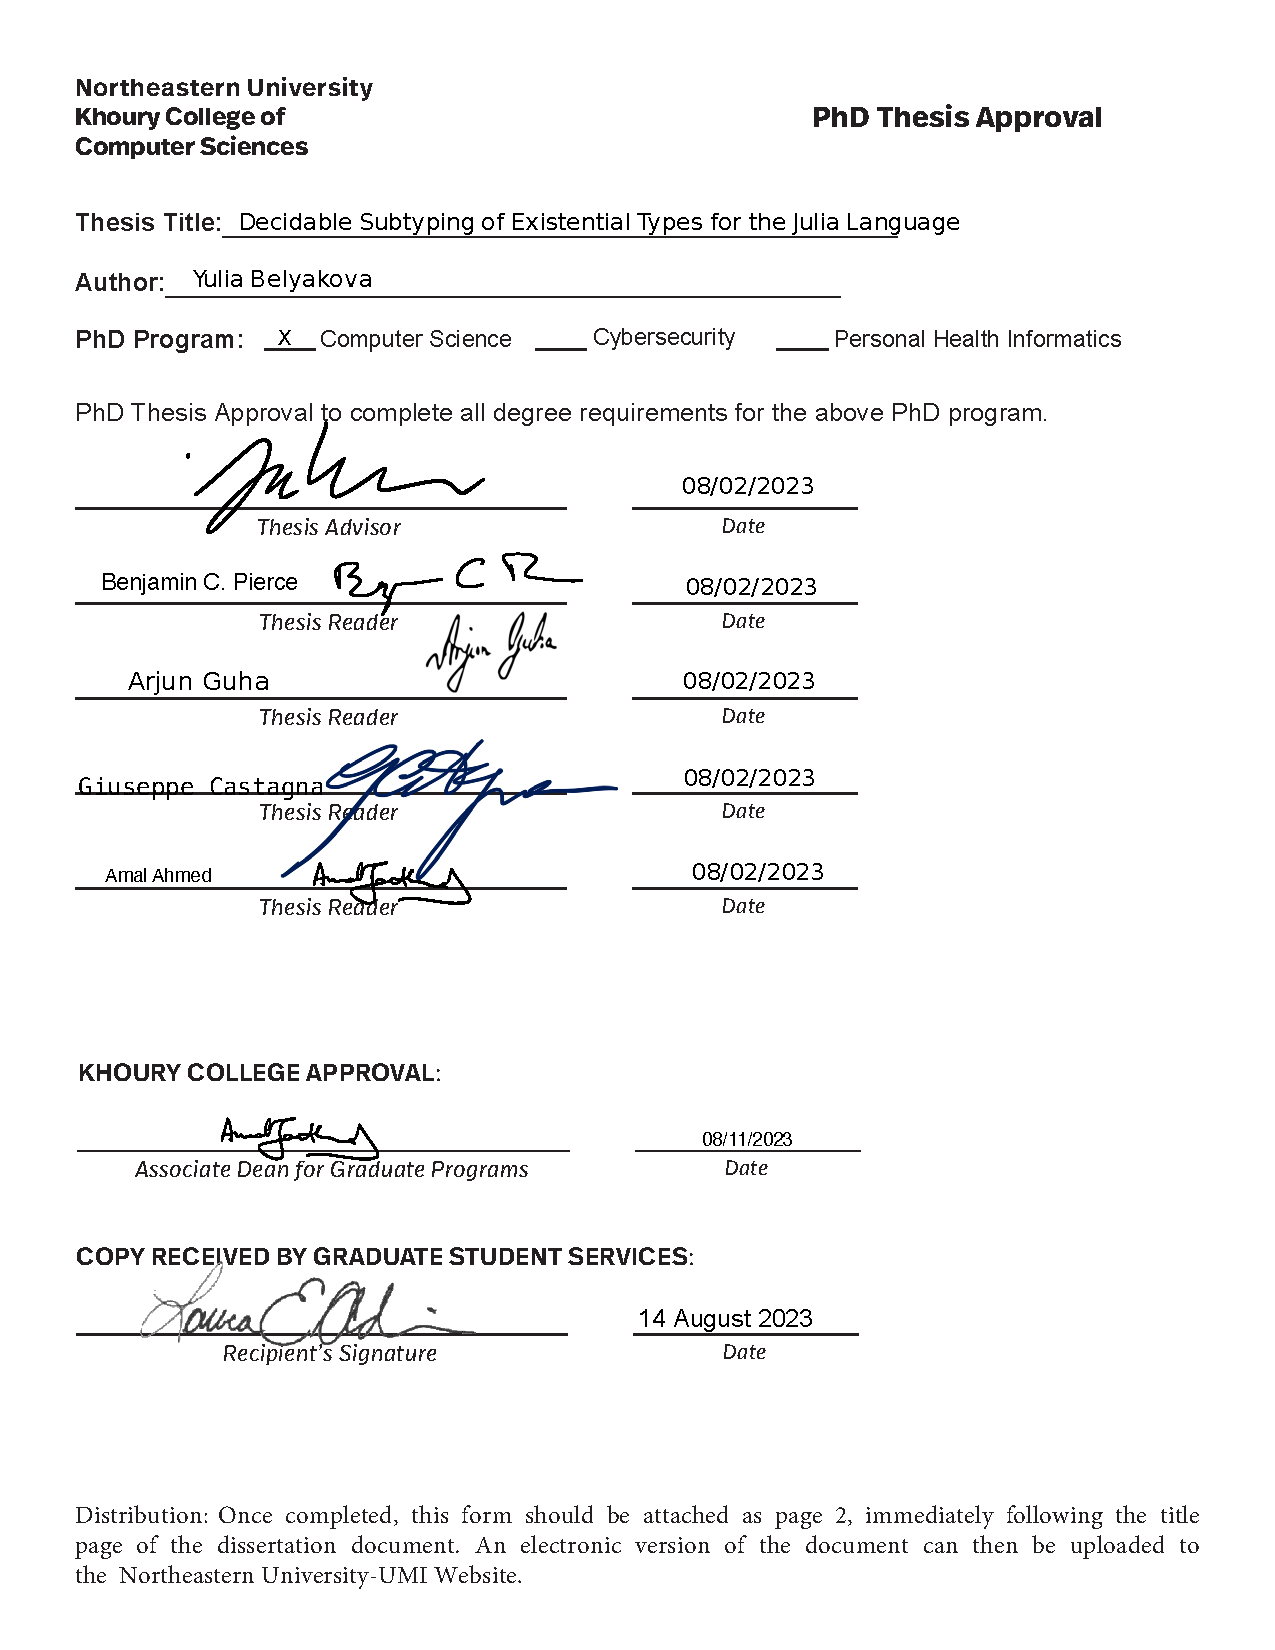
\includepdf[noautoscale]{approval.pdf}

\begin{abstract}

Julia is a dynamic, high-performance programming language
for scientific computing.
To encourage a high level of code reuse and extensibility, Julia is
designed around symmetric multiple dynamic dispatch, which allows functions
to have multiple implementations tailored to different argument types.
To resolve multiple dispatch, Julia relies on a subtype relation over a complex
language of run-time types and type annotations, 
which include set-theoretic unions, distributive tuples, parametric invariant 
types, and impredicative existential types.
Notably, subtyping in Julia is undecidable, which
manifests with a run-time stack-overflow error when program execution encounters
a subtyping query that causes the subtype checker to loop.

In this dissertation, I propose a decidable subtype relation for a restricted
language of Julia types where existential types inside invariant constructors
are limited to ones expressible with use-site variance.
To estimate migration effort that would be required for switching to the 
restricted type language, I analyze type annotations in the corpus of 9K
registered Julia packages.
Out of 2M statically identifiable type annotations in the corpus,
99.99\% satisfy the restriction, making it a viable candidate for
evolving Julia towards decidable subtyping.

\end{abstract}


\section{Proposal requirements}

The thesis proposal should include the relevant background materials from
literature and clearly specify the research problems to be attacked, the
techniques to be used, and a schedule of milestones towards completion.
Typically, the thesis proposal should not exceed 15 pages, excluding appendices
and bibliography.

\section{Outline}

\begin{enumerate}
  \item Introduction: overview of the problem and the proposal.
  \item Background: brief intro to Julia and an overview of types.
  \item Related work: wildcards and existential types, decidability of bounded
    quantification, union and intersection types.
  \item Research problems: what is the role of types and subtyping in Julia?,
    can we define a reasonable restriction on types to achieve decidable but
    still useful subtyping relation? (With a plan to attach the problems)
  \item Preliminary work: undesired properties of subtyping, confusion with
    diagonal types, tag-based semantic subtyping, model of Julia's JIT.
  \item Schedule of milestones.
\end{enumerate}

\chapter{Introduction}

\TODO{NOTE: this is ``the first shitty draft'', i.e. completely unedited stream
of thought.}

Julia is a dynamic, high-level language for scientific computing.
Its primary paradigm is \emph{multiple dynamic dispatch}, which allows for
high code reuse and extensibility. Although Julia does not have a static type
system, it does have an expressive language of types: both concrete user-defined
types that describe values, and abstract types that can be used in method type
annotations to specify multiple dispatch. Dispatch is implemented using
subtyping in this language of types.
The language of types is surprisingly complex, and there is no clean
specification of subtyping available to Julia users. The only reference is
effectively the implementation of subtyping, which is written in obscure C (or
C++?) code and meant to be efficient. The implementation is not very readable,
and the reason it needs to be fast is that subtyping is used at run-time.
As any function call in Julia is a dynamically dispatched call, and dispatch
relies on subtyping, it needs to be fast.

However, even the most efficient implementation of subtyping is not enough to
make the language fast. Dispatched calls can hinder optimizations. Therefore,
Julia's JIT compiler tries to remove dispatched calls and perform further
optimizations. In doing so, Julia heavily relies on type inference at run-time.
When inferred types are precise enough to ``statically'' dispatch calls, the JIT
will do so. Again, this means that subtyping is used. But furthermore, the types
are used by the type inference algorithm to guide optimizations.

As the primary purpose of types in Julia at the surface level is to describe
behaviors, the language of types is an unusual one. For example, it provides
impredicative exsitential types with bounded quantification. Furthermore,
covariant tuples and unions are distributive in Julia, which is similar to
semantic subtyping. Additionally, Julia supports a special kind of existential
types to allow for a common use case of dispatched methods: so-called diagonal
rule, where an existential variable is allowed to be instantiated only with a
concrete type. Given all this, there are concerns of understandability and
properties of the type language and subtyping in Julia.

As the first step in understanding the language of types, we tried to reverse
engineer the implementation of subtyping and provide a more readable
specification. This work is reported in \TODO{OOPSLA 18}.
While we did come up with subtyping rules that describe subtyping, we found
several issues: for example, subtyping was not transitive. There were also
several bugs in the implementation of subtyping. Furthermore, we found that the
diagonal rule works in such a way that the meaning of a type changes depending
on a subtyping relation it is checked against.
Most importantly, subtyping turns out to be undecidable in Julia. This means
that in practice, the user may face with a stack overflow at run-time because
subtyping is used for dispatching.
Another problem is that the rules we provided are hard to reason about to prove
transitivity, for example.
Thus, our first goal is to develop a specification of subtyping that is
decidable and can be reasoned about.

The way existential types are used in Julia are reminiscent of models of Java
wildcards. The key difference is that Julia's existential types are
impredicative. Interestingly, in the hope to avoid undecidability, Julia
developers intentionally restricted bounded quantification to, for example,
forbid recursive constraints on type variables.
Thus, some approaches to making subtyping decidable are not applicable, e.g.
material-shape separation \TODO{understand and explain}.

Ideally, subtyping should also be intuitive for the users. So we explore the
applicability of a semantic subtyping approach to the type language. We will
identify a property that we call tag-based semantic subtyping, and we will
strive to support this property.

Because efficiency is important for Julia, and the way it is achieved is by JIT
compilation, we explore the role of types in the JIT compiler. It turns out that
the JIT heavily relies on type inference \TODO{OOPSLA 21}. Therefore, we need to
understand what happens with types and which operations needs to be supported on
types. This will be our final guiding principle.


\end{document}
